\documentclass[
 openright,
 %twoside, % beidseitig für Druck
 a4paper
]{scrreprt}
%scrreprt
%% HTW Dresden Corporate Design
%% Copyright (C) Falk-Jonatan Strube <falkjonatanstrube@gmail.com>, 2017
%%% === Anfang Paket htwscr ===
\makeatletter
\ifcsname KOMAoption\endcsname%
%\KOMAoption{footheight}{11mm}	% mehr Platz für Wasserzeichen o.ä. in der Fußzeile
\recalctypearea	% s.o.
\RequirePackage{geometry}
\geometry{
	top=25mm, 
	bottom=25mm, 
	%headsep=10mm, 
	inner=25mm, 
	outer=25mm, 
	%footskip=15mm, 
	marginparsep=2mm
}
\RequirePackage{helvet}	% Corporate Design schreibt Arial/Helvetica vor
\renewcommand{\familydefault}{\sfdefault}	% s.o.
\RequirePackage{graphicx}	% für Grafiken
\RequirePackage{xcolor}		% für Farben
\definecolor{htworange}{RGB}{249,155,28}	% Corporate Design orange CMYK(0/45/100/0)
\definecolor{htwblue}{RGB}{0,116,188}			% Corporate Design blau CMYK(90/50/0/0)
\definecolor{htwgrey}{RGB}{128,128,128}		% Corporate Design gray 60% Schwarz [Annahme: CMYK(0,0,0,60)]
\RequirePackage{ifthen,xifthen}	% für Bedingungen/Optionen
\RequirePackage{etoolbox}				% s.o.

%%% Format des HTW-Headers (wird hier als Texteelement verwenden) nach dem Style der PowerPoint-Vorlagen. Weiterhin inspiriert durch das Paket tudscr (Corporate Design der TU Dresden)
%%% Dateipfad des Logos abhängig von der Verwendung als Paket/Input
\ifdefined\@isHTWCDpackage%
	\gdef\@pathtoimage{HTW}%
\else%
	\ifdefined\pathtomaster%
		\gdef\@pathtoimage{\pathtomaster /HTW}%
	\else 
		\gdef\@pathtoimage{htwcd/HTW}%
	\fi%
\fi%
\newcommand{\pathtologo}[1]{\gdef\@pathtoimage{#1}}
%%% Berechnung der Größe des Logos
\newlength{\htwLogoHeight}
\setlength{\htwLogoHeight}{12mm}	% Mindesthöhe des Logos laut Corporate Design: 11mm
\newlength{\@htwLogoWidth}
\AtBeginDocument{
\def\printLogo{\includegraphics[height=\htwLogoHeight]{\@pathtoimage}}
\setlength\@htwLogoWidth{\widthof{\printLogo}}
}
%%% Definition des Header
\newcommand{\@htwheader}{{\noindent%
%%% Header ist abhängig von dem Vorhandensein von department, institute und chair
\newcommand{\hasDepInsCh}{\gdef\@hasDepInsCh{}}%
\ifdefined\@department\hasDepInsCh\fi%
\ifdefined\@institute\hasDepInsCh\fi%
\ifdefined\@chair\hasDepInsCh\fi%
\begin{minipage}[b][\htwLogoHeight]{\dimexpr \textwidth - \@htwLogoWidth - 2mm \relax}% 2mm Abstand zwischen Logo und Linie
{\small{\bfseries%
\ifdefined\@faculty\@faculty{}\fi} %
\strut}%
{\color{htworange}\hrule height 1pt}%
\vspace{.1mm}%
\end{minipage}
\hfill%
\begin{minipage}[b][\htwLogoHeight]{\@htwLogoWidth}
\includegraphics[height=\htwLogoHeight]{\@pathtoimage}
\end{minipage}
\ifdefined\@hasDepInsCh%
\\%
\begin{minipage}{\textwidth}
\small%
\ifdefined\@department\@department{}\fi%
\ifdefined\@institute\ifdefined\@department,~\fi \@institute\fi%
\ifdefined\@chair\ifdefined\@department,~\else\ifdefined\@institute,~\fi\fi\@chair\fi\strut
%{\color{htworange}\hrule height 0.5pt}
\end{minipage}
\fi
}}

%%% Definition der Fußzeilen
\usepackage{scrlayer-scrpage}
\@ifclassloaded{scrreprt}{%
\renewcommand*{\partpagestyle}{scrheadings}
\renewcommand*{\chapterpagestyle}{scrheadings}%
}{}
\pagestyle{scrheadings}
% Definition der Seitenzahl-Position:

%\newif \if@twoside \@twosidefalse
%\if@twoside%
	%
%\else%
	% Beim einseitigen Dokument Seitenzahl auch außen/rechts.
%	\ofoot{\pagemark}%
%	\cfoot{}%
%\fi%  

%%% Einstellungen
\newcommand{\simpledate}{\gdef\@simpledate{}}		% Datum nicht mit "Eingereicht am:" Vorsatz
\newcommand{\nouppercase}{\gdef\@nouppercase{}}	% Titel/Parts/Chapters usw. nicht in Großbuchstaben

%%% Einiges erst zu Beginn des Dokumentes ausführen, um Einstellungen zu berücksichtigen
\AtBeginDocument{
\renewcommand\SS{SS}	% fix big ß
%%% Sektionen usw. ggf. in Großbuchstaben:
\providecommand{\chapterlinesformat}[3]{}	% compatibility
\providecommand{\chapterlineswithprefixformat}[3]{}	% compatibility
\providecommand{\sectionlinesformat}[4]{}	% compatibility
\ifdefined\@nouppercase\relax\else
\renewcommand\sectionlinesformat[4]{\@hangfrom{\hskip#2 #3}{\MakeUppercase{#4}}}
\@ifclassloaded{scrreprt}{%
\renewcommand\chapterlinesformat[3]{\@hangfrom{#2}{\MakeUppercase{#3}}}
\renewcommand\chapterlineswithprefixformat[3]{\MakeUppercase{#2#3}}%
}{}
\fi
%%% Anpassung der Part-Seite
\renewcommand*{\partheadstartvskip}{\@htwheader\vspace*{30mm}}
\renewcommand*{\raggedpart}{\raggedright}
\renewcommand*{\partformat}{\huge\ifdefined\@nouppercase \partname~\thepart\else\MakeUppercase{\partname~\thepart}\fi.}
\ifdefined\@nouppercase\setkomafont{part}{\Huge}\else\setkomafont{part}{\Huge\MakeUppercase}\fi
}

\newcommand{\bilingual}[3]{\ifdefined #1 \let #1\undefined\fi\newcommand{#1}{\iflanguage{english}{#3}{#2}}}	% Übersetzung von einigen Variablen in mehrere Sprachen

\newcommand{\checkThesis}[2]{\ifthenelse{\equal{#1}{diss}\OR\equal{#1}{doctoral}\OR\equal{#1}{phd}}{
\gdef#2{\dissertationname}}{
\ifthenelse{\equal{#1}{diploma}}{
\gdef#2{\diplomathesisname}}{
\ifthenelse{\equal{#1}{master}}{
\gdef#2{\masterthesisname}}{
\ifthenelse{\equal{#1}{bachelor}}{
\gdef#2{\bachelorthesisname}}{
\ifthenelse{\equal{#1}{student}}{
\gdef#2{\studentthesisname}}{
\ifthenelse{\equal{#1}{evidence}}{
\gdef#2{\studentresearchname}}{
\ifthenelse{\equal{#1}{project}}{
\gdef#2{\projectpapername}}{
\ifthenelse{\equal{#1}{seminar}}{
\gdef#2{\seminarpapername}}{
\ifthenelse{\equal{#1}{term}}{
\gdef#2{\termpapername}}{
\ifthenelse{\equal{#1}{research}}{
\gdef#2{\researchname}}{
\ifthenelse{\equal{#1}{log}}{
\gdef#2{\logname}}{
\ifthenelse{\equal{#1}{report}}{
\gdef#2{\reportname}}{
\ifthenelse{\equal{#1}{internship}}{
\gdef#2{\internshipname}}{
\ifthenelse{\equal{#1}{lecture}\OR\equal{#1}{lesson}\OR\equal{#1}{pract}}{
\bilingual{\professorname}{Vorlesung von}{Lecture by}
\simpledate
\gdef\@islecture{\relax}
\ifthenelse{\equal{#1}{lecture}}{\gdef#2{\lecturename}}{
\ifthenelse{\equal{#1}{lesson}}{\gdef#2{\lessonname}}{
\gdef#2{\practname}
}}}{
\gdef#2{#1}}}}}}}}}}}}}}}}

%%% Textfragmente der Titelseite in deutsch und englisch
\bilingual{\dateofbirthname}{Geboren am:}{Born on:}
\bilingual{\placeofbirthname}{in}{in}
\bilingual{\coursename}{Studiengang:}{Course:}
\bilingual{\disciplinename}{Studienrichtung:}{Discipline:}
\bilingual{\matriculationnumbername}{Matrikelnummer:}{Matriculation number:}
\bilingual{\matriculationyearname}{Immatrikulationsjahr}{Matriculation year:}
\bilingual{\graduationname}{zur Erlangung des akademischen Grades}{to achieve the academic degree}
\bilingual{\refereename}{Gutachter}{Referee}
\bilingual{\advisorname}{Fachreferent}{Advisor}
\bilingual{\supervisorname}{Betreuer}{Supervisor}
\bilingual{\professorname}{Betreuender Hochschullehrer}{Supervising professor}
\bilingual{\datename}{Eingereicht am:}{Submitted on:}
%% Thesis Typen (inspiriert von dem Paket tudscr):
\bilingual{\dissertationname}{Dissertation}{Dissertation} % diss, doctoral, phd 
\bilingual{\diplomathesisname}{Diplomarbeit}{Diploma Thesis} % diploma 
\bilingual{\masterthesisname}{Master-Arbeit}{Master Thesis} % master 
\bilingual{\bachelorthesisname}{Bachelor-Arbeit}{Bachelor Thesis} % bachelor 
\bilingual{\studentthesisname}{Studienarbeit}{Student Thesis} % student 
\bilingual{\studentresearchname}{Großer Beleg}{Student Research Project} % evidence 
\bilingual{\projectpapername}{Projektarbeit}{Project Paper} % project
\bilingual{\seminarpapername}{Seminararbeit}{Seminar Paper} % seminar
\bilingual{\termpapername}{Hausarbeit}{Term Paper} % term
\bilingual{\researchname}{Forschungsbericht}{Research Report} % research 
\bilingual{\logname}{Protokoll}{Log} % log 
\bilingual{\reportname}{Bericht}{Report} % report
\bilingual{\internshipname}{Praktikumsbericht}{Internship Report} % internship 
\bilingual{\lecturename}{Vorlesungsmitschrift}{Lecture Notes} % lecture 
\bilingual{\lectureauthorname}{Mitschrift von}{Notes by} % lecture  
\bilingual{\lessonname}{\"Ubungsmitschrift}{Lesson Notes} % lecture  
\bilingual{\practname}{Praktikumsmitschrift}{Pracital Course Notes} % lecture 
%%% Variablen für die Titelseite (inspiriert von dem Paket tudscr):
\renewcommand{\subject}[1]{\checkThesis{#1}{\@subject}}
\newcommand{\faculty}[1]{\gdef\@faculty{#1}}
\newcommand{\department}[1]{\gdef\@department{#1}}
\newcommand{\institute}[1]{\gdef\@institute{#1}}
\newcommand{\chair}[1]{\gdef\@chair{#1}}
\newcommand{\authormore}[1]{\gdef\@authormore{#1}}
\newcommand{\dateofbirth}[1]{\gdef\@dateofbirth{#1}}
\newcommand{\placeofbirth}[1]{\gdef\@placeofbirth{#1}}
\newcommand{\course}[1]{\gdef\@course{#1}}
\newcommand{\discipline}[1]{\gdef\@discipline{#1}}
\newcommand{\matriculationnumber}[1]{\gdef\@matriculationnumber{#1}}
\newcommand{\matriculationyear}[1]{\gdef\@matriculationyear{#1}}
\newcommand{\thesis}[1]{\checkThesis{#1}{\@thesis}}
\newcommand{\graduation}[2][]{\gdef\@graduation{#2}\gdef\@graduationshort{#1}}
\newcommand{\supervisor}[1]{\gdef\@supervisor{#1}}
\newcommand{\referee}[1]{\gdef\@referee{#1}}
\newcommand{\advisor}[1]{\gdef\@advisor{#1}}
\newcommand{\professor}[1]{\gdef\@professor{#1}}
%%% Titelseite (inspiriert von dem Paket tudscr):
\renewcommand*{\maketitle}{%
\begin{titlepage}%
\begin{flushleft}
\renewcommand{\thefootnote}{$\star$}%
%%% Kopfzeile HTW-Style:
\@htwheader\\[13mm]
%%% Die Zeilen für titlehead, subject, title, subtitle und author sind immer vorhanden (spacing)
{\noindent\@titlehead{}\strut}\\[3mm]%
{\Large\@subject{}\strut}\\[8mm]%
{\Huge\bfseries%
\ifdefined\@nouppercase\@title{}\else\MakeUppercase{\@title{}}\fi%
\strut}\\
{\Large\bfseries%
\ifdefined\@nouppercase\@subtitle{}\else\MakeUppercase{\@subtitle{}}\fi%
\strut}\\[11mm]
\ifdefined\@islecture\strut\else{\Large\@author{}\strut}\fi % Autor wird bei Vorlesungsmitschrift unten angezeigt
%%% Weitere Felder werden nur angezeigt, wenn sie definiert wurden
\ifdefined\@authormore\ifdefined\@islecture\else\\\fi{\@authormore{}\strut}\fi
\ifdefined\@dateofbirth\\\dateofbirthname{} \@dateofbirth{} \ifdefined\@placeofbirth\placeofbirthname{} \@placeofbirth{}\strut\fi\fi
\ifdefined\@course\\\coursename{} \@course{}\strut\fi
\ifdefined\@discipline\\\disciplinename{} \@discipline{}\strut\fi
\ifdefined\@matriculationnumber\\\matriculationnumbername{} \@matriculationnumber{}\strut\fi
\ifdefined\@matriculationyear\\\matriculationyearname{} \@matriculationyear{}\strut\fi
\ifdefined\@thesis\\[10mm]{\LARGE\bfseries
\ifdefined\@nouppercase\@thesis{}\else\MakeUppercase{\@thesis{}}\fi
\strut}
\ifdefined\@graduation\\[2mm]{\graduationname{}\strut}
\\[5mm]{\LARGE\bfseries
\ifdefined\@nouppercase\relax\else\MakeUppercase{\fi%
\@graduation{} \ifdefined\@graduationshort(\@graduationshort{})\fi
\ifdefined\@nouppercase\relax\else}\fi\strut}\fi\fi
\vfill\noindent
\ifdefined\@islecture\\[1mm]{\lectureauthorname{}\strut}\\[.7mm]{\Large\@author{}\strut}\fi
\ifdefined\@referee{\refereename{}\strut}\\[.7mm]{\Large\@referee{}\strut}\fi
\ifdefined\@advisor\\[1mm]{\advisorname{}\strut}\\[.7mm]{\Large\@advisor{}\strut}\fi
\ifdefined\@supervisor\\[1mm]{\supervisorname{}\strut}\\[.7mm]{\Large\@supervisor{}\strut}\fi
\ifdefined\@professor\\[1mm]{\professorname{}\strut}\\[.7mm]{\Large\@professor{}\strut}\fi
\ifdefempty{\@date}{}{\ifdefined\@simpledate\\[6mm]\relax\else\\[3mm]\datename{}~\fi\@date{}\strut}
\ifdefempty{\@publishers}{}{\\[4.5mm]{\Large\@publishers{}\strut}}%
\renewcommand\footnoterule{}
\@thanks\global\let\@thanks\@empty
\end{flushleft}
\end{titlepage}
\setcounter{footnote}{0}
}
\else%
\PackageError{htwcd}{htwcd needs a KOMA class!}%
\fi%
\makeatother
%%% === Ende Paket htwscr ===

% Vorgaben zum Seitenrand	
\geometry{
	top=30mm, 
	bottom=30mm, 
	%headsep=15mm, 
	inner=40mm, 
	outer=20mm, 
	%left=40mm,
	%right=20mm,
	%footskip=15mm,
}

\usepackage{scrlayer-scrpage}
\pagestyle{scrheadings}
\clearpairofpagestyles
\ofoot{\pagemark}
\raggedbottom

% Codierung
\usepackage[utf8]{inputenc}
\usepackage[T1]{fontenc}
\usepackage[ngerman]{babel}
\usepackage{csquotes}	% Anführungszeichen
\usepackage{amssymb}
\usepackage{pifont}

\newcommand{\cmark}{\ding{51}}
\newcommand{\xmark}{\ding{55}}

% Grafiken
\usepackage{graphicx}
\graphicspath{ {./images/} }
\usepackage{float}
\usepackage{longtable}
\usepackage{placeins}

% Tabellen
\usepackage{booktabs}
\usepackage{colortbl}
\usepackage{tabularx}
\usepackage{makecell}

\renewcommand\theadalign{bc}
\renewcommand\theadfont{\bfseries}
\renewcommand\theadgape{\Gape[4pt]}
\renewcommand\cellgape{\Gape[4pt]}

% Quelltext
\usepackage{listings}
\usepackage{scrhack}

% Links
\usepackage{xurl}
\usepackage[bookmarks,%
bookmarksopen=false,% Klappt die Bookmarks in Acrobat aus
colorlinks=true,%
linkcolor=black,%
citecolor=black,%
urlcolor=black,%
]{hyperref}
\usepackage{titleref}

\usepackage{datetime}


\usepackage{tikz}
\usetikzlibrary{positioning,shadings}
\usetikzlibrary{arrows}

% ======================================================
% Informationen für das Dokument und Titelseite:
% ======================================================
\faculty{Fakultät Informatik/Mathematik}

\title{Persönliche Daten in der Datenökonomie}

\author{
	Maria Mukian\\
	Philipp Steigler\\
	Eric Hans Gero Biele
}

\professor{Prof. Dr. Jürgen Anke}

\newdate{abgabe}{26}{01}{2022}
\date{\displaydate{abgabe}}
% ======================================================


% ======================================================
% Literatur/Quellen und Akronyme/Glossar:
% ======================================================
\usepackage[
backend=bibtex,
sortlocale=de_DE, 
bibencoding=utf8,
style=numeric, 
citestyle=numeric,
doi=false,
isbn=false,
url=false,
sorting=nty
]{biblatex}	% BibTeX
\bibliography{Bibliography}

\usepackage[acronym]{glossaries}
\makeglossaries
% ------------------------------------------
% Glossar  
% keine Umlaute im entry verwenden   
\newglossaryentry{natuerlichePersonG}
{
name={natürliche Person},
description={\glqq Eine natürliche Person meint den Menschen als Rechtssubjekt und somit als Träger von Rechten und Pflichten.\grqq{} \cite{NatPerson_2018}}
}

\newglossaryentry{webScrapingG}
{
name={Web-Scraping},
description={\glqq Web-Scraping ist das Schürfen von Daten, also die Datenextraktion aus Webseiten.\grqq{} \cite{webScraping_2021}}
}

\newglossaryentry{brokerG}
{
name={Broker},
description={\glqq Der Broker wirkt als Makler bei reiner Geschäftsvermittlung auf fremden Namen und auf fremde Rechnung (Abschlussvermittlung) oder als Kommissionär in eigenem Namen und auf fremde Rechnung.\grqq{} \cite{broker_2018}}
}

\newglossaryentry{smartContractsG}
{
name={Smart Contract},
description={\glqq Smart Contracts sind digitale Verträge, die in einer Blockchain gespeichert sind und automatisch ausgeführt werden, wenn vordefinierte Bedingungen erfüllt sind\grqq{} \cite{smartContract_2022}}
}

%============================================
% Akronyme
%============================================
\newglossaryentry{DSGVO}{
	type=\acronymtype, 
	name={DSGVO}, 
	description={Datenschutz-Grundverordnung}
}

\newglossaryentry{UN}{
	type=\acronymtype, 
	name={UN}, 
	description={United Nations}
}

\newglossaryentry{SaaS}{
	type=\acronymtype, 
	name={SaaS}, 
	description={Software as a Service}
}

\newglossaryentry{PaaS}{
	type=\acronymtype, 
	name={PaaS}, 
	description={Platform as a Service}
}
% ======================================================
\pagenumbering{roman}

\begin{document}
% ==============================================
% Deckblatt
% ==============================================
\maketitle

% ==============================================
% Abstract
% ==============================================
\setcounter{page}{1}
\pagenumbering{gobble}
\thispagestyle{empty}
\vspace*{5cm}
\begin{center}
\begin{minipage}{0.9\textwidth}
\chapter*{Abstract}

Die vorliegende Arbeit gibt einen Überblick über die Möglichkeiten der aktiven Monetarisierung von persönlichen Daten mit deren Potenzial und Einschränkungen. Im Zuge dessen wurden die Grundlagen der Datenökonomie, sowie der monetäre Wert von Daten untersucht und darauf aufbauend eine Fallstudie durchgeführt, welche die Basis dieser Arbeit bildet. Die Ergebnisse der Fallstudie führten zu einer Kategorisierung der Monetarisierungsmöglichkeiten durch den Verbraucher. Diese Arbeit ist sowohl für IT- und Wirtschaftswissenschaftler, als auch für Unternehmen und Verbraucher selbst interessant, die sich auf datengetriebene Technologien stützen.

\vspace*{1.5cm}
\end{minipage}
\end{center}
\clearpage

% ==============================================
% Verzeichnisse:
% ==============================================
% Inhaltsverzeichnis
\pagenumbering{roman}
\setcounter{page}{1}
\tableofcontents
% Abkürzungsverzeichnis
% ACHTUNG: Akronyme und Glossar muss (ähnlich wie bibtex) extra kompiliert werden über makeglossaries (in texmaker bspw. "makeglossaries %")
\printglossary[type=\acronymtype]
\addcontentsline{toc}{chapter}{Akronyme}
% Glossar
\printglossary[type=main]
\addcontentsline{toc}{chapter}{Glossar}
% Abbildungsverzeichnis
\listoffigures
\addcontentsline{toc}{chapter}{Abbildungsverzeichnis}
% Tabellenverzeichnis
\listoftables
\addcontentsline{toc}{chapter}{Tabellenverzeichnis}

% ==============================================
% Textteil
% Richtlinie: 25-40 Seiten
% \section{}, \subsection{}, \subsubsection{}
% ==============================================
\clearpage
\pagenumbering{arabic}
\chapter{Einleitung}
% * Einleitung
\section{Motivation}\label{Motivation}
Die Verbreitung des Internets auf Computern und mobilen Endgeräten hat zu einer Produktion riesiger Datenmengen geführt. Diese Daten -- insbesondere personenbezogene Daten -- haben sich zu einer wichtigen Ressource entwickelt, mit der Unternehmen einen Mehrwert erzeugen. Im Weiteren entstand daraus eine Datenökonomie, die allein auf dem Handel und der Verarbeitung personenbezogener Daten beruhen. \cite{humanDemand_2020} Dabei werden Daten meist jedoch nicht direkt von den Erzeugern, den individuellen Personen, verkauft. Stattdessen erheben große Internetdienste Anspruch auf die Daten ihrer Nutzer durch Klauseln in den Nutzungsbedingungen und verkaufen diese dann an Dritte weiter -- oftmals ohne Nutzer im Einzelfall darüber in Kenntnis zu setzen. Obwohl Individuen durch Erzeugung von Daten die Grundlage solcher Ökosysteme bilden, werden sie von Unternehmen bislang nur als Datenquelle gesehen und somit ausgenutzt. \cite{monetizingData_2016} \newline

\noindent Viele Personen werden sich in letzer Zeit allerdings zunehmend bewusst, dass Technologieunternehmen diese Daten sammeln und verkaufen. Darüber hinaus erkennen sie, dass ihre persönlichen Daten einen gewissen Wert haben und dass sie mehr Kontrolle über deren Verwendung haben sollten. Rantanen und Koskinen fanden in einer Studie heraus, dass Personen zwei wesentliche Forderungen an eine faire Datenökonomie stellen: transparente Kommunikation und eine aktive Rolle im Handel mit den eigenen Daten. Eine aktive Rolle an der Datenökonomie meint dabei, dass Individuen die Nutzung ihrer eigenen Daten kontrollieren und für die Teilnahme einen entsprechenden Gegenwert erhalten wollen. \cite{humanDemand_2020} \newline

\noindent Bereits im Jahr 2016 stellte Batineh et. al jedoch fest, dass es an Plattformen mangelt, auf denen Individuen als primäre Datenerzeuger ihre Daten für einen entsprechenden Gegenwert selbst anbieten können. \cite{monetizingData_2016}
% * Ziel und Methodik
\section{Ziel und Methodik}
Aus diesem Grund beschäftigen wir uns im Folgenden mit den verschiedenen Möglichkeiten für Personen, sich aktiv in der Datenökonomie zu beteiligen. In dieser Arbeit stellen wir dar, bei welchen Diensten individuelle Personen ihre Daten anderen Akteuren der Datenökonomie zur Verfügung stellen können und welchen Gegenwert sie dafür jeweils erhalten. Wir fokussieren uns dabei ausschließlich auf persönliche Daten, da diese sehr empfindliche Informationen über Individuen enthalten und deshalb für Unternehmen von großem Interesse sind. Zudem betrachten wir für jeden Fall, mit welcher Kontrolle und Transparenz die Daten geteilt werden. Unsere Forschungsfrage lautet deshalb:

\begin{center}
\textit{Welche Möglichkeiten gibt es für Personen, aktiv ihre persönlichen Daten ökonomisch zu verwerten?}
\end{center}

\noindent Um diese Frage zu beantworten beschäftigen wir uns zunächst mit den Begriffen \textit{personenbezogene Daten} und \textit{Datenökonmie}. Die Definition der Datenökonomie mit einer Abgrenzung zu anderen wirtschaftlichen Bereichen bildet die Voraussetzung für die darauffolgende Fallstudie. In dieser haben wir insgesamt sechs verschiedene Anbieter zur monetarisierung persönlicher Daten identifiziert. Obwohl die ausgewählten Unternehmen vielfältige Ziele verfolgen und sehr unterschiedlich funktionieren, lassen sie sich der Datenökonomie zuordnen. Nach Auswahl eines breiten Spektrums an Fallbeispielen analysieren wir jeden Dienst einzeln. Dabei gehen wir zunächst auf die Ziele der Anbieter ein und legen anschließend nachvollziehbar dar, wie Individuen der Datenökonomie ihre persönlichen Daten auf der jeweiligen Plattform monetarisieren können. Zusätzlich beschreiben wir in jedem Fall, welches Maß an Kontrolle und Transparenz den Benutzern offenbart wird. \newline

\noindent Im darauffolgenden Abschnitt werten wir die Ergebnisse der Fallstudie aus. Hierfür werden die Erkenntnisse zu den einzelnen Anbietern miteinander in Verbindung gebracht, um Gemeinsamkeiten und Unterschiede darzustellen. Im Mittelpunkt stehen dabei die Aspekte der Datenerhebung, Kontrolle und Transparenz über die Daten sowie der Gegenwert für Individuen. Dies ermöglicht uns abschließend, einige Themen -- wie beispielsweise die Ausnutzung von Personen -- kritisch zu hinterfragen und allgemeine Probleme abzuleiten. 

\chapter{Grundlagen}
% * Datenschutz
\section{Datenschutz}
\subsection{Personenbezogene Daten}
Laut der Definition in der Datenschutz Grundverordnung (\gls{DSGVO}) im Kapitel 1 Artikel 4 Nummer 1 werden personenbezogene Daten als diejenigen Informationen bezeichnet, mit denen sich \gls{natuerlichePersonG}en identifizieren lassen. Die Identifikation kann auf direktem oder indirektem Wege erfolgen, insbesondere durch die Zuordnung eines Namen zu Kennnummern, Standortdaten oder anderen psychischen, physiologischen, genetischen, wirtschaftlichen, kulturellen oder sozialen Merkmalen der natürlichen Person. \cite{DSGVO_Art4} Gemäß der europäischen Union werden Teilinformationen, die zusammen zur Identifizierung einer natürlichen Person dienen, ebenfalls als personenbezogene Daten kategorisiert. Werden diese Daten anonymisiert und lassen keinen Schluss auf die natürliche Person zu, so werden diese Daten nicht mehr als personenbezogen betrachtet. Beispiele für personenbezogene Daten sind Name, Vorname, Privatanschrift, E-Mail-Adresse mit Namen, Standortdaten sowie auch Informaionen zu persönlichen Interessen oder dem Konsumverhalten. Als nicht personenbezogene Daten werden beispielsweise Handelsregisternummer, anonymisierte E-Mail-Adressen und generell anonymisierte Daten betrachtet. \cite{PersBezDaten_2021} Ein Überblick zu den verschiedenen Arten von personenbezogenen Daten befindet sich in den Anlagen dieser Arbeit unter \ref{tab:personenbezogeneDaten}.

\subsection{Besonders schützenswerte personenbezogene Daten} \label{DSGVO_besonders}
Zu erwähnen ist, dass es besonders schützenswerte Daten einer natürlichen Person gibt. Die Verarbeitung dieser Daten ist entsprechend der DSGVO grundsätzlich untersagt. Zu diesen Daten gehören mitunter die rassische und ethnische Herkunft, politische Meinungen, religiöse oder weltanschauliche Überzeugungen, die Gewerkschaftszugehörigkeit, sowie genetische und biometrische Daten, Gesundheitsdaten oder Daten zum Sexualleben oder der sexuellen Orientierung einer natürlichen Person. Die im Artikel 9 Absatz 2 der DSGVO beschriebenen Fälle bilden die Ausnahme zur Verarbeitung dieser Daten. \cite{DSGVO_Art9}
% * Datenökonomie
\input{Kapitel_Grundlagen/Datenökonomie.tex}
% * Wert der Daten
\section{Der ökonomische Wert von personenbezogenen Daten}

Die Studie \textit{Ökonomischer Wert von Verbraucherdaten für Adress- und Datenhändler}, welche im Auftrag des Bundesministeriums der Justiz und für Verbraucherschutz durchgeführt wurde, ermittelte annäherungsweise den ökonomischen Wert von Nutzerdaten. Sie analysierten dafür die zehn umsatzstärksten Unternehmen Deutschlands im Bereich Datenhandel mit personenbezogenen Daten. Allein 2014 erwirtschafteten diese zehn Unternehmen einen Gesamtumsatz von etwa 450 Mio. Euro, wobei die Schufa beispielsweise im Besitz von 797 Mio. Einzeldaten zu 66,4 Mio. Personen ist. Das bedeutet im Umkehrschluss, dass die Schufa, bei einer Einwohnerzahl von 83,2 Mio. Menschen in Deutschland (Stand 2021 \cite{einwohnerzahl_2021}), Daten von knapp 80\% der deutschen Bevölkerung hat, wobei auf jeden Einzelnen durchschnittlich zwölf Einzeldaten entfallen. Die Studie kommt zu dem Ergebnis, dass der durchschnittliche Wert eines Datensatzes 0,86 Euro beträgt. Ein Datensatz wird dabei aus Post- und E-Mailadressen beziehungsweise Personendaten erstellt, die mit personenbezogenen Merkmalen, wie Konsumverhalten, Bonität, etc., angereichert sind. Bei einer Verwertbarkeit eines Datensatzes von 30 Jahren erzielten die untersuchten Unternehmen damit einen durchschnittlichen Umsatz von 26 Euro pro personenbezogenen Datensatz, wobei dieser je nach Unternehmen zwischen vier und 77 Euro schwankt. \cite{Wert_der_Daten_2017}

\chapter{Fallstudie}
% * Erklärung zur Auswahl der Fallbeispiele
\input{Kapitel_Fallanalyse/Erklärung.tex}
% * Payback
\section{Payback} \label{Payback}
Payback GmbH ist die Tochtergesellschaft der Lovalty Partner GmbH, welche wiederum ein Teil der American Express Gruppe ist. \cite{Payback_Info} Payback ist allgegenwärtig in Deutschalnd bekannt, entweder per Kundenkarte oder per App, mit welcher sich Punkte sammeln lassen. \newline
\noindent Payback wurde im Jahre 2000 gegründet und existiert in Deutschland, Italien, Indien, Polen, Mexiko und Österreich. \cite{Payback_Info} \newline

\subsection{Ziel}
In vielen teilnehmenden Einzelhandelsketten wird an der Kassse beim bezahlen nach Payback gefragt. Payback ist dabei ein Truepunkteprogramm (Paybackprogramm) mit dem Kunden bei jedem Einkauf Punkte sammeln können. Dies ist ganz einfach zu erklären, Payback hat über 600 Vertragspartner offline wie online, bei denen mit jedem Einkauf Punkte gesammelt werden können. Dabei kann der Kunde entweder seine Payback Karte vorlegen und diese einscannen lassen oder über das Smartphone die App vorzeigen, um Punkte zu sammeln. \cite{Payback} \newline

\noindent Das Ziel des Karten- bzw. Appinhabers ist dabei viele Punkte zu sammeln, um diese in Coupons und Prämien umtauschen zu können. Womit er für andere Produkte am Ende weniger bezahlen muss. \newline

\noindent Das Ziel von Payback ist es Daten zu generieren, um diese auswerten zu können, z. B. um das Kaufverhalten zu analysieren und dem Kunden dahingehend personalisierte Werbung zu zeigen. Ein weiteres Ziel ist es Verbraucher zu animieren mehr Geld auszugeben, als sie es ohne Rabatte oder Coupons getan hätten. \cite{web}


\subsection{Rollen, Datenfreigabe und -verarbeitung}
Mit der Recherche zu Payback ließen sich drei Rollen heraus kristallisieren, die für das Netzwerk von Payback von Interesse sind. Diese sind im nachfolgendem Fett markiert.\newline
Teilnehmen dürfen nur \textbf{Nutzer} die ihr 16. Lebensjahr vollendet, sowie eine natürliche Person sind und ihren Wohnsitz im europäischen Wirtschaftsraum haben.\cite{Payback_Teilnahme} Das beudeutet Unternehmen sind nicht berechtigt als Nutzer Punkte bei Einkaufen zu sammeln. Möchte der Nutzer nun am Programm teilnehmen, benötigt Payback persönliche Daten, sogenannte Basisdaten. Basisdaten sind:\newline
- Namen\newline
- Geburtsdatum\newline
- Anschrift.\newline
 Ohne diese Daten können zwar Punkte gesammelt werden, allerdings können diese nicht eingelöst werden. Weiterhin besteht die Möglichkeit freiwillig mehr, als die Basisdaten anzugeben. Dies bedeutet der Nutzer fungiert somit als Datenquelle für Payback.

 Payback stellt dabei den \textbf{Verein} dar, welcher alle Daten sammelt, analysiert und aufbereitet. Zum Beispiel verarbeitet es die Basisdaten und die freiwilligen Angaben für die Anmeldung und die Abwicklung. Nebst werden die Richtigkeit und die Vollständigkeit der Adressdaten überprüft, damit postalisch Werbung an den Kunden zugesandt werden kann. Die Daten und ggf. der vom Nutzer vorgenommenen Änderungen der Basisdaten werden auch an die \textbf{Partnerunternehmen} übermittelt, dies gilt nur für das Unternehmen woher der Kunde die Kundenkarte erhalten hat. Eine Ausnahme bildet die Apotheke, dahin werden die Daten nicht übermittelt. Für weitere Übermittlungen an Dritte oder Partnerunternehmen finden nur statt, wenn diesen gesondert vom Nutzer zugestimmt wurden. 

Sobald der Kunde einen Einkauf tätigt, meldet das Partnerunternehmen die Kundennummer und Rabattdaten an Payback.  Ausnahme bildet hier wieder die Apotheke. \newline

\noindent In Absprache mit den Partnerunternehmen stellt Payback Coupons und Prämien zur Verfügung. Diese können von den Nutzern aktiviert werden. Sobald der Nutzer diesen einlöst übermittelt Payack an das Partnerunternehmen, dass diese beim bezahlen berücksichtigt werden.

Weiterhin werden Kommunikationsdaten übermittelt, dies sind alle Angaben, die über das Kundenterminal oder über das Service Center, zur Bearbeitung eines Anliegens des Kunden anfallen. \newline

\noindent Der Nutzer kann entscheiden, ob seine Daten für Zwecke der Marktforschung und Werdbung verwendet werden dürfen. Wenn der Nutzer einwilligt, werden passende werbliche Angebote für Ihn ausgewählt. Diese erfolgen durch die Auswertung der Daten zur Mustererkennung im Einkaufsverhalten. Die Angebote werden entweder postalisch oder per eMail oder per SMS mitgeteilt. Diese Daten werden an Payback und die Partnerunternehmen zum Zwecke für Werbung verarbeitet. Der Kunde hat dabei jederzeit die Möglichkeit die Einwilligung zu widerrufen. Sobald die Einwilligung zur Verarbeitung der Daten für Werbezwecke vorliegt, wird anhand dessen ebenfalls eine Werbeplanung und Erfolgskontrolle durchgeführt. \newline

\noindent Payback speichert die Daten der Kunden, solange diese aktiv am Programm teilnehmen, anschließend werden diese gelöscht. Steuerrechtlich werden diese jedoch 10 Jahre lang aufbewahrt. Die Kommunikationsdaten, zum Beispiel bei Kontaktierung des Service Centers werden nach sptestens 6 Jahren gelöscht.
\cite{Payback_Datenschutz}



\subsection{Daten auf Payback monetarisieren}
Der monetäre Wert für die Nutzerdaten lässt sich nicht in Zahlen bestimmen. 
\noindent Es besteht lediglich die Möglichkeit für den Nutzer die gesammelten Punkte in Coupons und Prämien umzustauschen. Dabei hat der Nutzer die Kontrolle darüber, wie viele Punkte er einlösen möchte. Hierbei sei zu erwähnen, dass bei der normalen Payback Karte die gesammelten Punkte eines jeden Jahres zum 30.09 verfallen, wenn diese nicht verwertet werden. 
Eine weitere Möglichkeit besteht darin, sobald mindestens 200 Punkte erreicht wurden, kann der Nutzer sich diese auf sein Konto auszuahlen lassen. Dabei entsprechen die 200 Punkte einem Betrag von 2€. \cite{Payback_Teilnahme} \newline

\noindent Payback bietet 3 Kartenmodelle für das Punktesammelsystem an. Zum einen die PAyback Karte, welche dauerhaft kostenlos ist, sowie das der Kunde bei allen Vertragspartnern Punke sammeln können. Das zweite Modell ist die Payback American Express Karte, welche ebenfalls kostenlos ist. Hierbei kann der Kunde bei jeder Bezahlung mit dieser Karte Punkte sammeln sei es bei der Bezahlung von Einkäufen bei Partnerunternehmen sowie nicht Partnerunternehmen. Der Vorteil ist bei dieser Karte, dass die Punkte nicht verfallen können und es gibt sogar extra 5000 Payback Punkte bei Kartenabschluss. Die Payback Visa Karte ist das dritte Modell, diese besitzt ebenfalls kein Punkteverfall. Weitere Vorteile dieser Karte sind 0€ Jahresgebühr, 0€ Gebühren bei Bargeldabhebung und auch außerhalb von Partnerunternehmen kann der Kunde bei Bezahlung mit der Karte Punkte generieren. 
Durch diese drei Kartenmodelle hat der Nutzer die Wahl, in welcher Form er am Bonusporgramm teilnehmen möchte und zu welchen Konditionen.
Positiv sei zu erwähnen das Payback einen TÜV geprüften Datenschutz besitzt. \cite{Payback_Karten} 
% * Kaufland
\section{Kaufland Card}
Die Kaufland Card ist eine Vorteilskarte für die Einzelhandelskette Kaufland. Die Kaufland Card existiert seit dem 28.10.2021 in Deutschland, wurde aber zuvor schon 2019 in Osteuropa eingeführt.

\subsection{Rollen und Ziele}
Kaufland verfolgt mit der Einführung der Kaufland-App das Ziel, den Einkaufsprozess zu digitalisieren und somit zu vereinfachen. Darunter zählen beispielsweise digitale Preisschilder, digitale Kassenbons, kontaktloses Bezahlen aber auch die Kaufland Card. \cite{Kaufland_Ziele} Mit der Kaufland Card sollen Kunden an das Unternehmen gebunden und das Kaufverhalten der Nutzer verstanden werden, um somit relevante und personalisierte Werbung zu präsentieren. \cite{Kaufland_Datenschutz} Folglich gibt es zwei Rollen: \newline

\noindent \textbf{Kunde:} Der Kunde kann sich einerseits eine digitale Kaufland Card in der Kaufland-App oder andererseits eine klassische Kaufland Card in einer Filiale verschaffen, um somit am Bonusprogramm teilnehmen zu können. Damit hat er die Möglichkeit, Treuepunkte für einen Einkauf zu bekommen, Sparangebote und Coupons zu erhalten sowie an Gewinnspielen teilzunehmen. Für die Registrierung des Einkaufs und die Erfassung der Treuepunkte ist es dabei notwendig, den zur Kaufland Card zugehörigen Barcode beim Bezahlen vorzuzeigen. \newline

\noindent \textbf{Kaufland:} Kaufland fungiert bei diesem Bonusprogramm einerseits als Datenkonsument, welcher die Daten der Kunden sammelt und verarbeitet aber andererseits auch als Serviceanbieter, welcher die gesammelten Daten analysiert und die Inhalte auf den Nutzer zuschneidet. Damit will Kaufland den Einkaufsprozess vereinfachen und eigene Angebote bewerben bzw. hervorheben.

\subsection{Datenerhebung}
Bei der Registrierung für die Kaufland Card benötigt Kaufland folgende Daten: E-Mail Adresse oder Mobilfunknummer, Name, Geschlecht, Geburtsdatum und Adresse. Darüber hinaus werden die Einkaufsdaten bei dem Vorzeigen des Barcodes erhoben. Das bedeutet, dass der Kunde selbst die Wahl hat, ob sein Einkauf registriert wird und damit seine Einkaufsdaten erhoben werden. Entscheidet sich dieser jedoch gegen das Vorzeigen des Barcodes, wird damit auch die Teilnahme am Bonusprogramm verwehrt. Für den Kunden besteht jedoch die Möglichkeit die registrierten Einkäufe und Kassenbons in der Kaufland-App einzusehen -- nicht jedoch sie zu bearbeiten oder zu löschen. Dies ist nur durch die Löschung des gesamten Kundenkontos möglich. \cite{Kaufland_FAQ} Bezüglich des Datenschutzes und der zusammengehörigen Datenverarbeitung garantiert Kaufland sich an die geltenden Datenschutzbestimmungen zu halten und sie nicht an Dritte weiterzugeben. \cite{Kaufland_Rechtliches} 

\subsection{Daten bei Kaufland monetarisieren}
Die Erhebung von Einkaufsdaten bildet die Grundlage für Kaufland, dem Nutzer mit der Kaufland Card einen Gegenwert anzubieten. Dieser umfasst einerseits exklusive Preisnachlässe für ausgewählte Artikel und andererseits Prämien, die durch den Eintausch gesammelter Treuepunkte erhältlich sind. Einen Treuepunkt erhält man pro fünf Euro Einkaufswert, welcher nach einem Jahr wiederum verfällt. Eine Umwandlung der Punkte in Geld ist allerdings mit der Kaufland-App nicht möglich. \cite{Kaufland_FAQ} Zusammengefasst bedeutet das, dass folgende Schritte für die Monetariserung der Daten notwendig sind:

\begin{enumerate}
	\item Bei Kaufland registieren (App oder Filiale) 
	\item Personenbezogene Daten hinterlegen
	\item Alter für die Teilnahme verifizieren (Teilnahmealter: mind. 18 Jahre)
	\item Barcode bei einem Einkauf vorzeigen
	\item Punkte einlösen
\end{enumerate}

% * Shoop
% \input{Kapitel_Fallanalyse/Shoop.tex}
% * BitaAboutMe
\section{BitsAboutMe}
BitsAboutMe ist ein in der Schweiz ansässiges Unternehmen, welches eine Plattform bereitstellt, auf der personenbezogene Daten verwaltet und gleichzeitig verkauft werden können.

\subsection{Ziel}
Als Ziel setzt sich das Unternehmen, den Nutzern mehr Kontrolle über die eigenen Daten zu geben. Damit soll ein fairer Datenhandel zwischen Datenkonsumenten und Datenanbietern sowie eine aktive Teilnahme an der Monetarisierung geschaffen werden. Außerdem lädt das Unternehmen noch weitere Unternehmen dazu ein, an diesem Netzwerk teilzunehmen und bietet unterschiedliche Analyse- und Auswertungsmöglichkeiten, sowie eine Schnittstelle zu den Datenanbietern an. Damit soll das Wachstum des Netzwerkes und die Nutzungsmotivation gesteigert werden, um einen positiven \gls{netzwerkeffektG} der Plattform zu erreichen.

\subsection{Rollen bei BitsAboutMe}
\textbf{Nutzer:} Nutzer können auf der Plattform, ähnlich wie im folgenden Abschnitt \ref{invisibly} bei Invisibly, ihre Daten von diversen Konten, wie Instagram, Facebook, Spotify, Amazon aber auch E-Mail- und Bankkonten hinzufügen (Abbildung \ref{fig:bitsaboutmeDatenquellen}), wobei der Nutzer zusätzlich einen Steckbrief über sich selbst ausfüllen kann. Neben dem Verkauf von persönlichen Daten soll ein Überblick über die Daten des Nutzers an einem zentralen Ort verschafft werden. Der Nutzer kann durch den Import verschiedener Datenquellen herausfinden, wie das eigene Nutzungsverhalten in sozialen Netzwerken ist, wie groß der eigene CO\textsubscript{2}-Fußabdruck ist oder ob man einen gesunden Lifestyle führt. Um damit nur einige Möglichkeiten zu nennen, hat der Nutzer also damit die Möglichkeit, die Daten der jeweiligen Datenquellen einzusehen, aggregiert darzustellen und sich auswerten zu lassen. \newline

\noindent Der Nutzer fungiert demzufolge als Datenanbieter beziehungsweise Datenquelle, wobei jedoch die Privatsphäre im Vordergrund steht. BitsAboutMe garantiert durch eine Verschlüsselung der Datenbank auf Nutzerebene und einem Rechenzentrum in der EU oder in der Schweiz für eine hohe Sicherheit und eine ausschließliche Einsicht der Daten durch den Nutzer selbst. Dieser kann mithilfe der \gls{PWA} stets selbst entscheiden, welche Daten konkret freigegeben werden und welche nicht.\newline

\noindent Genauer betrachtet, hat der Nutzer die Möglichkeit, einzelne Datensätze der verlinkten Datenquelle auf \textit{Geheim} oder \textit{Privat} zu stellen oder sogar zu löschen. Die Einstellung \textit{Privat} ist dabei die Standardeinstellung und bedeutet, dass die Daten in die Analysen einbezogen werden und auf dem Marktplatz (Abbildung \ref{fig:bitsaboutmeMarktplatz}) angeboten werden können. Die Einstellung \textit{Geheim} dagegen verhindert die Veröffentlichung der Daten auf dem Marktplatz, sowie das Einbeziehen dieser in die Analysen. Wird ein Datensatz gelöscht, so wird er gänzlich aus der verlinkten Datenquelle entfernt.

\begin{figure}[!ht]
	\centering
	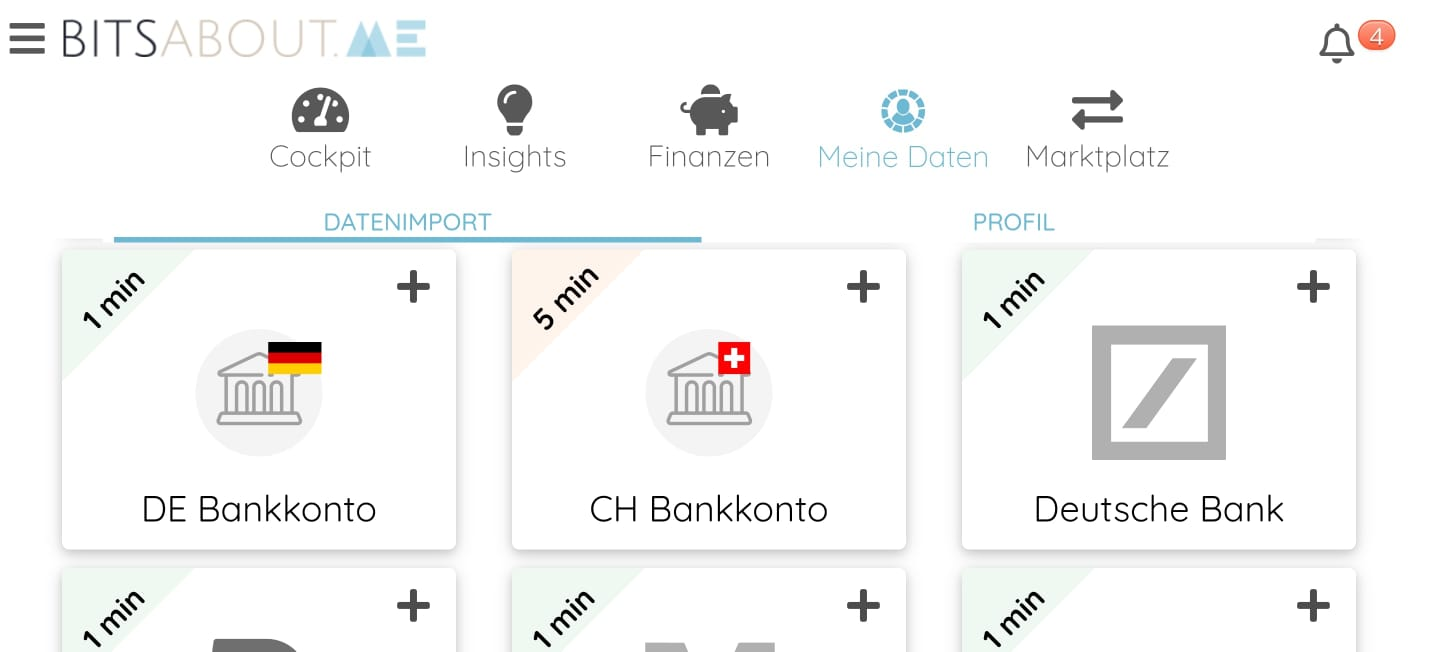
\includegraphics[width=\textwidth]{bitsaboutme_datenquellen}
	\caption{Möglichkeiten des Hinzufügens von Datenquellen auf der BitsAboutMe-Plattform mit annähernder Zeitabschätzung}
	\label{fig:bitsaboutmeDatenquellen}
\end{figure}
\FloatBarrier

\noindent \textbf{Käufer:} Käufer auf der BitsAboutMe-Plattform sind Unternehmen, welchen BitsAboutMe eine SaaS-Lösung anbietet, mit der sie als Datenkonsumenten die bereitsgestellten Daten von Nutzern erwerben können und Überblick über stattgefundene Transaktionen erhalten.

\subsection{Daten auf der BitsAboutMe-Plattform monetarisieren}
Damit der Nutzer die persönlichen Daten nun monetarisieren kann, bietet er eine Auswahl der Daten auf dem Datenmarktplatz an. BitsAboutMe verfolgt dabei eine getrennte Architektur vom persönlichen Datenspeicher (im Folgenden \textit{PDS} genannt) und dem persönlichen Daten-Marktplatz (im Folgenden \textit{PDM} genannt). Das bedeutet, dass die Daten bei dem Verknüpfen der Konten mit der BitsAboutMe-Plattform vorerst verschlüsselt im PDS abgelegt werden, worauf der Nutzer alleinig zugreifen kann. Entschließt dieser sich nun zu einem Verkauf dieser, so werden diese anonymisiert und an den PDM transferiert, sodass durch den Nutzer ausgewählte Datenkonsumenten beziehungsweise Unternehmen Zugriff auf das Datenprofil haben. Durch das Teilen des Datenprofils verdient der Nutzer Geld. Zusätzlich erhält BitsAboutMe ebenfalls eine Gebühr für die Transaktion.\newline

\noindent Möchte der Nutzer jedoch zukünftig nicht mehr sein anonymisiertes Datenprofil zur Verfügung stellen, so ist eine Rücknahme oder eine Löschung des Datenprofils jederzeit möglich. \newline

\begin{figure}[!ht]
	\centering
	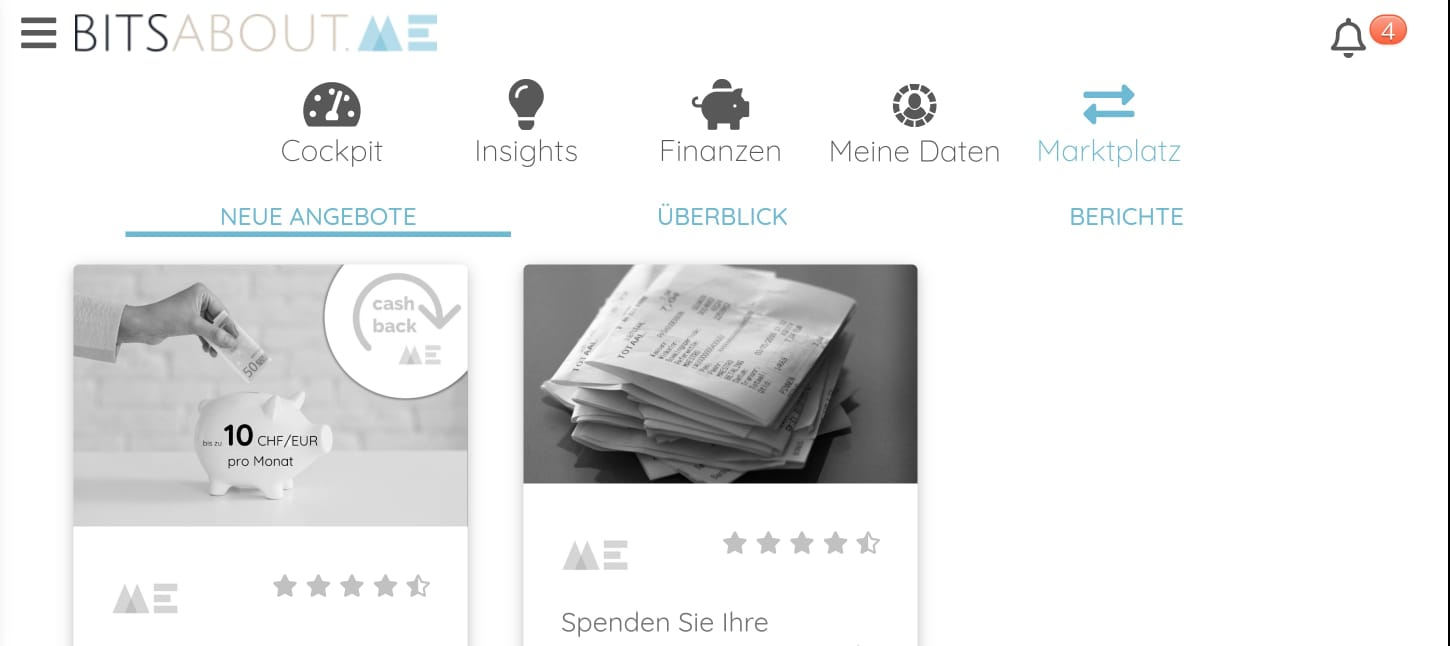
\includegraphics[width=\textwidth]{bitsaboutme_marktplatz.jpg}
	\caption{Persönlicher Datenmarktplatz auf der BitsAboutMe-Plattform mit Angeboten, angenommener Angebote und Informationen zu abgerufenen Daten}
	\label{fig:bitsaboutmeMarktplatz}
\end{figure}
\FloatBarrier

\noindent Neben dem Teilen des Nutzerprofils bietet die Plattform noch eine weitere Möglichkeit an, Daten anonym zu monetarisieren: Der Nutzer kann von ihm erhaltene Kassenzettel einscannen und erhält 1\% Cashback auf den jeweiligen Einkauf. Dies ist jedoch auf 10€ im Monat begrenzt. Diese Daten fließen ebenfalls in das persönliche Benutzerprofil ein, da BitsAboutMe anhand dessen analysiert, wie nachhaltig und gesund der Nutzer lebt und gleichzeitig einen Überblick über die Finanzen schafft. Damit die Daten valide und brauchbar für die Datenkonsumenten sind, werden die Kassenbons mit den Zahlungen des hinterlegten Bankkontos abgeglichen. Nur auf Zahlungen, die auf dem Bankkonto durchgeführt wurden, gibt es Cashback. Unternehmen können diese Daten folglich erwerben und für die Marktforschung und andere, im Abschnitt \ref{datenoekonomie} Datenökonomie, beschriebene Zwecke nutzen. \newline

\noindent Zusammengefasst sind folgende Schritte für die Monetariserung der Daten notwendig:
\begin{enumerate}
	\item Registrieren
	\item Datenquellen verbinden
	\item (digitale Identität prüfen)
	\item PDM aktivieren
	\item Daten freigeben und Geschäft abschließen
\end{enumerate}
% * Datum
\section{Datum}
Datum ist ein Netzwerk, in dem Nutzer ihre Daten dezentralisiert in einer Blockchain speichern können. Darüber hinaus ermöglicht es dem Nutzer diese Daten zu kaufen oder verkaufen und die Nutzung dieser entsprechend einzuschränken. Es ist also nicht nur ein Speicherort für Daten, sondern dient auch als Online-Datenmarktplatz.

\subsection{Ziel}
Datum zielt mit dem Projekt darauf ab, die im Kapitel \ref{Motivation} beschriebenen Anforderungen der Nutzer an ihre Daten umzusetzen beziehungsweise zu berücksichtigen. Das heißt, das Unternehmen möchte dem Nutzer einerseits eine sichere Datenspeicherung auf einer \gls{smartContractsG}-Blockchain ermöglichen (siehe Abbildung \ref{fig:datumBlockchain}) und andererseits die aktive Teilnahme am Verkauf ihrer oder seiner Daten ermöglichen. Dabei hat der Nutzer volle Kontrolle darüber wie die Daten genutzt werden und mit wem sie geteilt werden. Weiterhin soll dem Nutzer ermöglicht werden jederzeit die übertragenden Daten einsehen zu können, um somit Transparenz, sowie eine ständige Nachvollziehbarkeit über den Zugriff auf die Daten zu schaffen. \newline

\noindent Daraus resultieren zusammengefasst folgende sechs Anforderungen, die das Unternehmen mit ihrem Projekt aus Nutzersicht definiert hat:
\begin{enumerate}
	\item Die Daten werden quellseitig verschlüsselt
	\item Die Daten sind unveränderbar
	\item Die Daten können monetarisiert werden
	\item Die Daten werden dezentralisiert gespeichert
	\item Die Daten werden anonymisiert
	\item Der Nutzer besitzt die Kontrolle darüber, welche Daten genutzt werden, wie lange die Daten genutzt werden und wie die zukünftige Verwendung der Daten erfolgt 
\end{enumerate}

\noindent Aus Käufersicht möchte das Unternehmen eine gute Datenqualität garantieren, indem die Daten der Nutzer validiert werden, um somit verlässliche und aussagekräftige Daten für Prognosen oder andere Verwendungszwecke zu liefern. Dafür soll sich auf das Datum-Netzwerk verlassen werden und im Zusammenhang damit ein \textit{Trust-Ranking-System} implementiert werden. Das heißt, es soll zukünftig eine Bewertungsmöglichkeit zur Qualität der angebotenen Daten geben, um somit ein Ranking für besonders vertrauenswürdige Quellen erstellen zu können. Für die konkrete Validierung der Daten schlägt das Unternehmen stattdessen weitere externe Validierungsdienste wie \textit{Civic} oder \textit{uPort} vor, um beispielsweise Identitäten verifizieren zu können.

\begin{figure}[!ht]
	\centering
	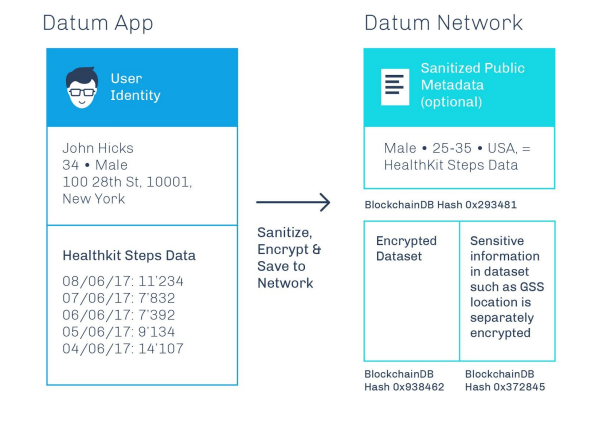
\includegraphics[width=\textwidth]{datum_blockchain}
	\caption{Bereinigung und Speicherung von HealthKit-Daten in der Smart Contract-Blockchain \cite{datum_2017}}
	\label{fig:datumBlockchain}
\end{figure}

\subsection{Rollen im Datum-Netzwerk}
\textbf{Nutzer:} Nutzer sind diejenigen Personen im Netzwerk, die ihre persönlichen oder geschäftlichen Daten hinterlegen und zum Verkauf anbieten können. Sie nehmen somit die Rolle des Datenanbieters ein. Datum ermöglicht dem Nutzer zudem eine Einflussnahme auf die Privatsphäreeinstellungen, sodass folgende fünf Einstellungen getroffen werden können: 
\begin{enumerate}
	\item Das Teilen der Daten ist nicht erlaubt
	\item Das Teilen der Daten ist nur mit ganz bestimmten, identifizierten und dem Nutzer bekannten Datenkonsumenten gestattet
	\item Das Teilen der Daten ist wiederum nur mit ganz bestimmten, identifizierten und dem Nutzer bekannten Datenkonsumenten, gestattet, aber für eine Mindestgebühr
	\item Die Daten sind für jeden verfügbar
	\item Die Daten sind für jeden verfügbar aber für eine Mindestgebühr
\end{enumerate}

\noindent \textbf{Käufer:} Käufer können sich im Datum-Netzwerk den Zugriff auf die Daten der Nutzer erkaufen. Sie fungieren in diesem Netzwerk demzufolge als Datenkonsumenten, wobei sie jedoch nur einen eingeschränkten Zugriff auf die Daten haben, und zwar entsprechend der Nutzungsbedingungen des Nutzers. Auch sie können unterschiedliche Informationen offenlegen:
\begin{enumerate}
	\item Identität des Käufers
	\item Die allgemeine Datenschutzerklärung
	\item Die Zweckmäßigkeit
	\item Die Dauer der Aufbewahrung der Daten
	\item Das \textit{Datum-Network-Trust-Rating}
\end{enumerate}

\noindent \textbf{DAT-Token-Holder:} DAT-Token-Holder steuern das Netzwerk und ermöglichen Transaktionen in dem Netzwerk. Die DAT-Token selbst dienen als Währung, um Daten kaufen, verkaufen oder überhaupt speichern und anbieten zu können. Der Wert eines DAT-Token liegt aktuell bei 0,000070€. (Stand: 20.01.2022 \cite{DAT_Token_price}) \newline

\noindent \textit{Hinweis: Auf weitere Rollen, wie beispielsweise Storage Nodes wird im Folgenden nicht eingegangen, da sich diese vorwiegend mit der technischen Komponente einer Blockchain befassen und im Sinne der Datenökonomie weniger relevant sind.}

\subsection{Daten im Datum-Netzwerk monetarisieren}
Nun stellt sich wiederum die Frage, wie die Nutzer ihre Daten aktiv verkaufen und somit zu Geld machen können. Dafür sieht das Netzwerk folgendes Protokoll vor: \newline

\noindent Zuerst muss der Nutzer seine Daten mit der Client-Software (Android- oder iOS-App) dem Netzwerk preisgeben. Diese werden jedoch davor verschlüsselt, wodurch nur der Nutzer selbst Zugriff auf die Daten hat. Die verschlüsselten Daten werden daraufhin an mehrere \textit{Storage Nodes} gesendet und sind damit repliziert. Nun kann ein Datenkonsument sein Interesse für die veröffentlichten Daten eines Nutzers äußern. Daraufhin erhält der Nutzer, also der Datenanbieter, eine Kaufanfrage für die übermittelten Konditionen des Datenkonsumenten. Ist er damit einverstanden, kann der Datenanbieter das Angebot annehmen. Ebenso kann dieser auch ein Gegenangebot an den Datenkonsumenten schicken. Kommt ein Geschäft zustande, so sendet der Datenkonsument DAT-Token als Gegenwert an den Nutzer, welcher im Gegenzug den Schlüssel zur Entschlüsselung seiner Daten oder einem Teil seiner Daten veräußert.
Das Geschäft kann dabei als Einmalkauf abgewickelt werden oder in Form eines Abonnements. \cite{datum_2017} \newline

\noindent Die folgende Abbildung verdeutlicht dies noch einmal:

\begin{figure}[!ht]
	\centering
	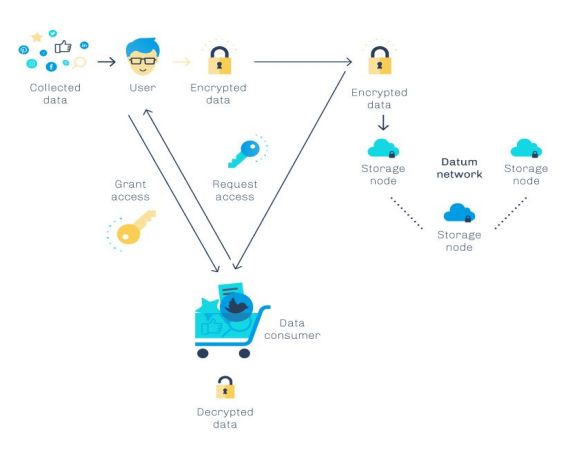
\includegraphics[width=\textwidth]{datum_scheme}
	\caption{Schema einer Kaufabwicklung im Datum-Netzwerk \cite{datum_2017}}
	\label{fig:datumScheme}
\end{figure}
\FloatBarrier
% * Invisibly
\section{Invisibly}
Invisibly ist eine Plattform, bei der Benutzer ihre persönlichen Daten zur lizenzierten Freigabe bereitstellen können. Sie befindet sich derzeit noch in der Beta-Phase und ist bisher ausschließlich in Amerika verfügbar.

\subsection{Hintergrund und Ziel}
Die Plattform hatte ursprünglich das Ziel, bezahlungspflichtige Artikel leichter zugänglich zu machen. Benutzer der Webseite sollten Werbung ansehen und dafür Token erhalten, welche sie anschließend für den Zugang zu einzelnen Publikationen von Nachrichtenseiten und Wissenschaftsmagazinen ausgeben konnten -- ohne bei den einzelnen Diensten beispielsweise ein Abonnement abzuschließen. Da diese Idee nur wenige Personen überzeugte, wurde das Konzept überarbeitet. \cite{techRadarInvisibly_2021} \newline

\noindent Heute verfolgt Invisibly das Ziel, seine Benutzer mit einem fairen Anteil am Wert zu beteiligen, der bei der Verarbeitung persönlicher Daten entsteht. Die Plattform versucht dies aktuell auf zwei verschiedene Wege. Im Gegensatz zu anderen Plattformen, die Inhalte strategisch platzieren, versucht Invisibly als erstes seinen Benutzern auf Basis der freiwillig geteilten Daten hochwertige Inhalte zu präsentieren, die sie tatsächlich sehen wollen: \begin{quote}
    We are creating an AI-powered platform with a feed that`s a true extension of you, rather than a feed strategically curated and targeted at you by the Big Tech and brands. \cite{invisiblyWhyPay_2021}
\end{quote} Im zweiten Schritt zielt Invisibly darauf ab, seine Benutzer direkt am Verkauf der persönlichen Daten zu beteiligen, indem sie ihnen regelmäßig Geld auszahlt. \cite{invisiblyWhyPay_2021} Der Gründer von Invisibly, Jim McKelvey, beschreibt seine Plattform in einem Interview wiefolgt: \begin{quote}
    We basically act as your agent. We try to sell you to advertisers and we give you the money. We ask how much you are willing to sell, package it up and sell it to the highest bidder. \cite{techRadarInvisibly_2021}
\end{quote} Die Plattform verkauft die Rohdaten ihrer Nutzer jedoch nicht direkt -- stattdessen lizenziert Invisibly die Daten ihrer Nutzer. Auf diese Weise bleibt die individuelle Person Eigentümer der Daten und kann selbst bestimmen, welche Daten sie freigeben möchte. \cite{invisiblyGetPaid_2021} Anschließend vermittelt Invisibly die Lizenzen an Werbetreibende für Dienste und Produkte, die am besten zum jeweiligen Benutzer passen. Sie erhalten mit einer Lizenz solange Zugriff auf die persönlichen Daten, bis ein Benutzer seine Lizenz widerruft und somit die Freigabe beendet. Der Vorteil für Unternehmen besteht darin, dass Invisibly sie durch den Kauf von Lizenzen mit den Individuen zusammenbringt, die potentiell am besten zu deren Produkten passen. \cite{techRadarInvisibly_2021} Dabei ist es wichtig zu erwähnen, dass Benutzer von Invisibly ihre Daten freiwillig zur Lizenzierung freigeben und deshalb wahrscheinlich von einer Vermittlung an Dritte nicht abgeneigt sind. \newline

\noindent Im Folgenden wird erklärt, wie Individuen ihre persönlichen Daten bei Invisibly zu Geld machen können.

\subsection{Daten monetarisieren}
Benutzer sammeln bei Invisibly Punkte, indem sie persönliche Daten mit der Plattform teilen. Gesammelte Punkte werden anschließend in US-Dollar umgerechnet und ausgezahlt. Derzeit gibt es drei verschiedene Möglichkeiten, Punkte zu sammeln: \newline

\noindent \textbf{Datenquellen verlinken:} Die meisten Punkte sammeln Benutzer, indem sie verschiedene Datenquellen in ihrem Invisibly-Profil hinterlegen. Für jede Datenquelle wird monatlich ein fester Betrag an Punkten gutgeschrieben, ähnlich wie bei einem passiven Einkommen. \cite{pymntsInvisibly_2021} Das Verknüpfen eines Bankkontos wird beispielsweise mit \textit{75 Punkten} pro Monat vergütet, wobei Werbepartner so Zugriff auf sämtliche Transaktionsdaten erhalten. Andererseits lassen sich verschiedene soziale Netzwerke bei Invisibly hinterlegen. Für jeden Account erhält ein Benutzer monatlich \textit{25 Punkte} und es werden aktuell die Plattformen Instagram, Twitter, TikTok, LinkedIn und Pinterest unterstützt. Zum Schluss bietet Invisibly eine Browser-Erweiterung an, welche den Verlauf der besuchten Webseiten aufzeichnet. Mit ihr sammeln Benutzer \textit{200 Punkte} pro Monat. \cite{instagramInvisibly_2021, lifewireInvisibly_2021} \newline

\noindent \textbf{Fragen zur Person:} Benutzer können ihr Invisibly-Profil vervöllständigen, indem sie verschiedene Fragen zu ihrer Person beantworten. So fragt die Webseite beispielsweise nach dem Geschlecht, dem höchsten Bildungsabschluss oder ob man Kinder hat. Jede Antwort wird dabei mit \textit{einem Punkt} vergütet. \cite{instagramInvisibly_2021} \newline

\noindent \textbf{Persönliches Feed:} Das persönliche Feed ist Invisibly's Vision von einer besseren Alternative zu Facebook und ähnlichen Beispielen. Das Feed enthält relevante Beiträge, die auf Basis der freiwillig geteilten, persönlichen Daten von verschiedenen Datenquellen ausgewählt und angezeigt werden. Diese Beiträge bestehen aus Bildern mit kurzen Texten und verweisen auf Diensteleistungen und Produkte von Werbetreibenden, wie beispielsweise Gegenstände zum Kaufen, Reise- und Ausflugsziele, Veranstaltungen, Gutscheine oder sonstige Angebote in Online-Shops und vieles mehr. Jeder Beitrag kann mit einem \textit{Like} oder \textit{Dislike} markiert werden -- auf diese Weise sammelt Invisibly Daten über persönliche Interessen und kann Vorschläge noch besser auf jede Person zuschneiden. Benutzer erhalten im Gegenzug für jeden Like oder Dislike \textit{einen Punkt}, wobei die maximale Anzahl an Punkten hier auf 20 Punkte pro Tag begrenzt ist. \cite{invisiblyWhyPay_2021} \newline

\noindent Die gesammelten Punkte können abschließend direkt in Geld umgewandelt werden: 100 Punkte entsprechen \$1 und eine Auszahlung ist ab 500 Punkten möglich. \cite{invisiblyWhyPay_2021} Diese Monetarisierung bringt Invisibly's Nutzern derzeit ca. \$60 bis \$100 im Jahr, abhängig von der Anzahl verlinkter Datenquellen. Das liegt daran, dass aktuell ein flaches Bezahlmodell verwendet wird, bei dem jeder Nutzer gleich viel Geld bzw. Punkte für seine persönlichen Daten bekommt -- unabhängig davon, wieviel die Daten konkret für Werbetreibende wert sind. In Zukunft soll ein kompetitives Modell zum Einsatz kommen, bei dem Personen eine höhere Dividende erhalten, wenn die Daten für Werbetreibende mehr wert sind. \cite{pymntsInvisibly_2021} Der Gründer von Invisibly geht davon aus, dass ein schnell wachsender Marktplatz mit mehr Werbetreibenden und Individuen in wenigen Jahren bereits \$1000 pro Jahr für Nutzer des Dienstes erwirtschaften kann. \cite{techRadarInvisibly_2021} 

\chapter{Auswertung der Fallstudie}
\section{Ergebnisse}

\begin{table}[!ht]
\begin{tabular}[h]{ |l|c|c|c|c|c| }
    \hline
    \thead{} & \thead{Cashback} & \thead{Payback} & \thead{BitsAboutMe} & \thead{Datum} & \thead{Invisibly} \\
    \hline
    \makecell{\textbf{Transparenz\textsuperscript{1}}} & & & & & \\
    \makecell{Konsument} & & & \cmark & \cmark & \\
    \makecell{Zeitraum} & & & \cmark & \cmark & \\
    \makecell{Verwendungszweck} & & & \cmark & \cmark & \\
    \makecell{Umfang} & & & \cmark & \cmark & \\
    \hline
    \makecell{\textbf{aktive Teilnahme\textsuperscript{2}}} & & & & & \\
    \makecell{bewusste Freigabe} & & & \cmark & \cmark & \\
    \makecell{Rückruf möglich} & & & \cmark & \cmark & \\
    \hline
    \makecell{\textbf{Gegenwert\textsuperscript{3}}} & & & & & \\
    \makecell{Geld} & & & \cmark & \cmark & \\
    \makecell{Preisnachlass} & & & \xmark & \xmark & \\
    \makecell{Prämien} & & & \xmark & \xmark & \\
    \hline
    \makecell{\textbf{Datenerhebung\textsuperscript{4}}} & & & & & \\
    \makecell{First-Party} & & & \xmark & \xmark & \\
    \makecell{Second-Party} & & & \xmark & \xmark & \\
    \makecell{Third-Party} & & & \cmark & \cmark & \\
\end{tabular}
\caption{\label{tab:Auswertung der Fallstudie} Übersicht zur Auswertung der Fallstudie.}
\end{table}

\noindent \textsuperscript{1}Der Nutzer hat Einsicht über Art und Umfang der verarbeiteten Daten - unterteilt in nachfolgende Kategorien \newline

\noindent \textsuperscript{2}Der Nutzer nimmt aktiv an der Monetariserung seiner Daten teil - unterteilt in nachfolgende Kategorien \newline

\noindent \textsuperscript{3}Der Gegenwert, den der Nutzer für den Verkauf seiner Daten erhält - unterteilt in nachfolgende Kategorien\newline

\noindent \textsuperscript{4}Die Art der Datenerhebung aus Sicht des Datenkonsumenten gemäß Kapitel \ref{datenoekonomie} Datenökonomie - unterteilt in nachfolgende Kategorien\newline
\section{Diskussion der Ergebnisse}
Alle betrachteten Fälle der Fallstudie dienen dazu, dass Nutzer ihre Daten monetarisieren können. Auf unterschiedlichen Wegen werden Nutzer dazu motiviert, die analysierten Dienste zu nutzen. Denn nicht nur durch das Angebot der Datenmonetarisierung, sondern auch durch Analyseservices, der Erstellung eines Feeds und personalisierte Werbung versuchen die jeweiligen Dienste ihre Reichweite zu steigern. Es werden demzufolge stets weitere Anreize neben der Monetarisierung geschaffen, das Netzwerk oder den Dienst zu nutzen. Dabei rückt der Verkauf der Daten durch den Nutzer meist in den Hintergrund. So werben BitsAboutMe, Invisibly und Datum beispielsweise damit, wieder die volle Kontrolle über das digitale Leben zu erhalten. Dennoch wird sofort ersichtlich, dass auch Daten aktiv monetarisiert werden können. Kaufland und Payback dagegen werben primär mit Rabattaktionen und Prämien, um die Nutzungsmotivation der Verbraucher zu steigern. Die direkte Monetarisierung der personenbezogenen Daten heben beide Dienste dabei allerdings nicht hervor. Stattdessen geht es aus Sicht der Nutzer darum, Punkte zu sammeln und diese für Prämien oder Rabatte einzulösen. Daher kann angenommen werden, dass die Kenntnis der Nutzer über den Verkauf ihrer Daten limitiert ist und die Aufmerksamkeit von der Datenmonetarisierung abgelenkt wird. \newline

\noindent Darüber hinaus profitieren Payback und Kaufland von einem starken Lock-In-Effekt. Das meint, dass Punkte beispielsweise nicht zwischen anderen Bonusprogrammen übertragbar sind und somit Wechselbarrieren entstehen. Für den Nutzer ist dies weniger wünschenswert, da sie an die entsprechenden Dienste gebunden werden. Bei Kaufland ist dieser Effekt am stärksten zu beobachten, da Punkte und Rabatte lediglich auf dieses Unternehmen beschränkt sind. Payback dagegen bietet mit seinen 600 Online-Shops und 30 Partnern eine größere Auswahl und ermöglicht zudem die Auszahlung der Punkte. Ähnliches gilt für Invisibly, wo die gesammelten Punkte zum jetzigen Stand ausschließlich in bares Geld umgewandelt werden können. Als Gegenbeispiel sind dafür BitsAboutMe und Datum zu erwähnen. Bei BitsAboutMe werden Nutzer direkt mit Geld vergütet und im Datum-Netzwerk erhalten sie DAT-Token, welche auf beliebigen Kryptobörsen eintauschbar sind. \newline 

\noindent Bei der Monetarisierung der Daten spielt der Gegenwert für die Nutzer eine wichtige Rolle. Obwohl überwiegend direktes Geld als Gegenwert für die Daten geboten wird, lässt sich die Fairness des Datenhandels nicht bestimmen. Selbst mit dem im Kapitel \ref{oekonomischerWert} bestimmten Wert personenbezogener Daten lässt sich ein Vergleich nicht durchführen. Dies liegt mitunter an mangelnder Transparenz, sowie an dem Angebot und der Nachfrage auf der jeweiligen Plattform. Da BitsAboutMe, Invisibly und Datum sehr verschiedene Datenmarktplätze sind, lässt sich der Preis nicht konkretisieren. Hinzu kommt, dass die drei Dienste entweder noch im Anfangsstadium ihrer Entwicklung sind oder das Netzwerk noch nicht groß genug ist, um dies abschätzen zu können. Der Grund dafür ist ein indirekter Netzwerkeffekt: Der Wert des Netzwerks steigt durch das steigende Angebot von Nutzerdaten, was mehr Datenkonsumenten anlockt. Diese wachsende Konkurrenz und die steigende Nachfrage führen zu höheren Preisen und somit zu mehr Geld für einzelne Personen. \newline

\noindent Es ist positiv anzumerken, dass Individuen Möglichkeiten haben, ihre persönlichen Daten aktiv zu monetarisieren. Personen werden teilweise jedoch mit Prämien, Rabatten und Geld gelockt, sämtliche Daten über sich preiszugeben. Dabei besteht das Risiko, dass Personen voreilig bzw. unkontrolliert Daten mit Plattformen teilen, die sie danach nicht einfach widerrufen können. Diese Gefahr ist vor allem bei sensiblen persönlichen Daten hoch, beispielsweise bei Bankkonten oder Gesundheitsdaten. Des Weiteren beeinflussen Bonusprogramme das Konsumverhalten einiger Personen, indem sie mit Prämien und Rabatten zu falschen Kaufentscheidungen angeregt werden: Sie kaufen Produkte, die sie ohne Rabatte vielleicht nicht gekauft hätten. Grund dafür ist der Lock-In-Effekt, da Rabatte an bestimmte Produkte gebunden sind und eventuell verfallen, wodurch letztendlich der Gegenwert der monetarisierten Daten verfällt. \newline

\noindent Insgesamt ist die Intention einiger Dienste, Daten kontrolliert zu verkaufen, positiv zu bewerten. Auch der Ansatz persönliche Daten in einem festgelegten Rahmen zu lizenzieren klingt zunächst vielversprechend. Es muss jedoch festgehalten werden, dass die Betreiber der Plattformen den Missbrauch der Daten aus technischen Gründen nicht verhindern können. Denn die in Kapitel \ref{datenoekonomie} beschriebenen Eigenschaften von Daten zeigen, dass Daten beliebig oft ohne Wertverlust vervielfältig werden können. Das bedeutet beispielsweise, dass Datenkonsumenten erworbene Daten auch nach Ablauf der Vertragslaufzeit weiterverwenden oder zu ihren Gunsten weiterverkaufen können. Darüber hinaus werden andere Plattformen, wie beispielsweise Google, nicht davon abgehalten, weiterhin Daten über Individuen zu sammeln und verkaufen. Das bedeutet, dass Personen nicht die volle Kontrolle über ihre persönlichen Daten zurückerlangen, indem sie sich auf der Plattform anmelden. Die Plattformen verhindern nicht die Ausnutzung von Individuen durch Dritte -- vielmehr bieten sie nur einen zusätzlichen Dienst an, mit dem sich Personen aktiv an der Datenökonomie beteiligen können. Obwohl sich der Grad an Aktivität von Plattform zu Plattform etwas unterscheidet, bringen Individuen ihre persönlichen Daten selbst aktiv ein und erhalten dafür einen entsprechenden Gegenwert. Darüber hinaus sei noch erwähnt, dass Personen ihren Profit erhöhen können, indem sie sich bei mehreren Diensten gleichzeitig anmelden und somit ihre Daten mehrfach monetarisieren.


\chapter{Zusammenfassung}

% ==============================================
% Literaturverzeichnis
% ==============================================
\nocite{*}
\printbibliography
\addcontentsline{toc}{chapter}{Literaturverzeichnis}

% ==============================================
% Anhang
% ==============================================
\appendix
\chapter*{Anlagen} \label{Anlagen}
\begingroup
\begin{table}[!ht]
\renewcommand{\arraystretch}{1.5} % vertical padding
\begin{tabularx}{\textwidth}{| X | X |}
\hline
\rowcolor[rgb]{0.737,0.839,0.862}
\textbf{Kategorie} & \textbf{Personenbezogene Daten} \\
\hline
Soziodemografische/-ökonomische Angaben & Alter, Geschlecht, Bildung, Beruf, Einkommen, Familienstand etc. \\
\hline
Geografische Angaben & Standort, Anschrift etc. \\
\hline
Sensible Daten & Ethnische  Herkunft,  politische  Meinungen, Religions-
zugehörigkeit,  Gesundheitsdaten,  Sexualleben,  bio-
metrische Daten etc. \\ 
\hline
Persönlichkeitsprofil & Extraversion, Gewissenhaftigkeit etc. \\
\hline
Angaben über Konsumverhalten & Getätigte Einkäufe etc. \\
\hline
Interessen & Produkte, Marken, Musik, Film etc. \\
\hline
Technische Angaben & Browser, Endgerät, IP-Adressen, Nutzungs-/Surfverhalten (Web-Tracking), Cookies etc. \\
\hline
Werturteile & Schul-, Studienabschluss-, Arbeitszeugnisse, Diplome, Zertifikate, etc. \\
\hline
Audiovisuelle Daten & Videoaufzeichnungen, Fotos, Audio-Mitschnitte etc. \\
\hline
Biometrische Daten & Geschlecht, Haut-, Haar-, Augenfarbe, Statur, Kleidergröße, etc. \\
\hline
Indirekte bzw. personenbeziehbare Daten & Personalausweisnummer, Versicherungsnummer, Kreditkartennummer, Kfz-Kennzeichen, Telefonnummer, E-Mail-Adresse etc. \\
\hline
\end{tabularx}
\caption{Arten von personenbezogenen Daten (Angelehnt an: \textit{Ökonomischer Wert von Verbraucherdaten für Adress- und Datenhändler S.7} \cite{Wert_der_Daten_2017})}
\label{tab:personenbezogeneDaten}
\end{table}
\endgroup



\addcontentsline{toc}{chapter}{Anlagen}
\setcounter{chapter}{1}

% Endblatt (weiß)
\clearpage
\thispagestyle{empty}
\begin{center}
\vfill
\phantom{© \makeatletter\@author\makeatother}
\end{center}

\end{document}
